% SDRTerm — Iridium decoder pipeline walkthrough
%
% Build with:  pdflatex pipeline.tex
% (Twice, so ToC and cross-references resolve.)
%
% Uses: amsmath, amssymb, tikz, pgfplots, listings, hyperref, geometry
%       ── all standard TeXLive / MacTeX packages.

\documentclass[11pt,a4paper]{article}

\usepackage[margin=2cm]{geometry}
\usepackage{amsmath,amssymb,amsthm}
\usepackage{tikz}
\usepackage{pgfplots}
\pgfplotsset{compat=1.18}
\usetikzlibrary{arrows.meta, positioning, shapes.geometric, calc, decorations.pathreplacing}
\usepackage{listings}
\usepackage{xcolor}
\usepackage{hyperref}
\usepackage{caption}
\usepackage{booktabs}
\usepackage{siunitx}
\usepackage{parskip}

\hypersetup{
  colorlinks=true,
  linkcolor=blue!70!black,
  urlcolor=blue!60!black,
  citecolor=black,
}

\lstset{
  basicstyle=\ttfamily\small,
  frame=single,
  breaklines=true,
  showstringspaces=false,
  columns=fullflexible,
  keepspaces=true,
  backgroundcolor=\color{gray!5},
}

\title{Iridium Signal Capture and Processing\\
       \large A Mathematical Walkthrough of SDRTerm's iridium\_decoder Plugin}
\author{SDRTerm project}
\date{\today}

\begin{document}
\maketitle
\tableofcontents
\vspace{2em}

%═══════════════════════════════════════════════════════════════════
\section{Introduction}
%═══════════════════════════════════════════════════════════════════

The Iridium satellite constellation consists of 66 active low-earth-orbit
(LEO) satellites at approximately \SI{780}{km} altitude, providing global
voice and data service in the L-band. This document walks through the
complete signal chain used by SDRTerm's \texttt{iridium\_decoder} plugin
to turn raw radio-frequency samples into decoded Iridium messages. Each
stage is presented with its mathematical formulation, why it is needed,
and how it is implemented in the code.

The chain, from antenna to decoded message, consists of five stages:

\begin{center}
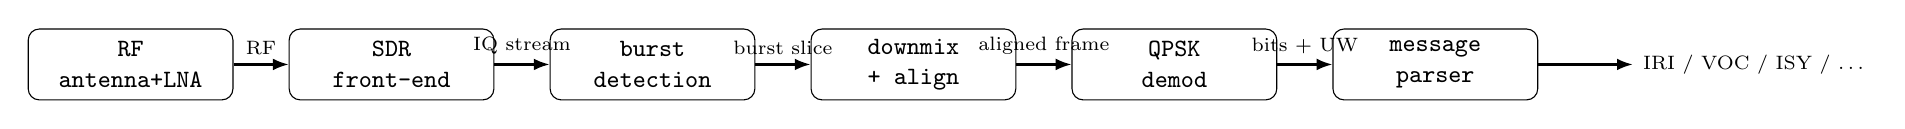
\begin{tikzpicture}[node distance=0.7cm,
  block/.style={draw, rounded corners, minimum width=2.6cm, minimum height=0.9cm,
                align=center, font=\small\ttfamily},
  arrow/.style={-{Latex[length=2mm]}, thick}]

  \node[block] (rf)      {RF\\antenna+LNA};
  \node[block, right=of rf]      (sdr)  {SDR\\front-end};
  \node[block, right=of sdr]     (det)  {burst\\detection};
  \node[block, right=of det]     (dmx)  {downmix\\+ align};
  \node[block, right=of dmx]     (dem)  {QPSK\\demod};
  \node[block, right=of dem]     (par)  {message\\parser};

  \draw[arrow] (rf)  -- node[above,font=\scriptsize]{RF}                (sdr);
  \draw[arrow] (sdr) -- node[above,font=\scriptsize]{IQ stream}         (det);
  \draw[arrow] (det) -- node[above,font=\scriptsize]{burst slice}       (dmx);
  \draw[arrow] (dmx) -- node[above,font=\scriptsize]{aligned frame}     (dem);
  \draw[arrow] (dem) -- node[above,font=\scriptsize]{bits + UW}         (par);
  \draw[arrow] (par.east) -- ++(1.2,0) node[right, font=\scriptsize]{IRI / VOC / ISY / \ldots};
\end{tikzpicture}
\end{center}

%═══════════════════════════════════════════════════════════════════
\section{Signal Basics}
%═══════════════════════════════════════════════════════════════════

\subsection{Complex baseband}

Any real-valued RF signal $s_{\text{RF}}(t)$ oscillating around a carrier
frequency $f_c$ can be written as
\begin{equation}
s_{\text{RF}}(t) \;=\; \mathrm{Re}\bigl[\, x(t)\, e^{j 2\pi f_c t} \bigr]
                 \;=\; I(t)\cos(2\pi f_c t) - Q(t)\sin(2\pi f_c t),
\end{equation}
where the \emph{complex baseband} representation is
\begin{equation}
x(t) \;=\; I(t) + j Q(t) \;\;\in\;\; \mathbb{C}.
\end{equation}

An SDR mixes the received RF signal down by $f_c$ (the ``tuner center'')
and delivers the complex baseband $x[n]$ as a stream of complex samples.
For the RTL-SDR the samples arrive as unsigned 8-bit I and Q bytes
interleaved (\texttt{cu8} format):
\begin{equation}
x[n] \;=\; \frac{I_{\text{byte}}[n] - 127.4}{128}
        + j\,\frac{Q_{\text{byte}}[n] - 127.4}{128}.
\end{equation}

\subsection{Sampling and Nyquist}

If the SDR samples at rate $f_s$, then $x[n] = x(n/f_s)$. Nyquist tells us
we can unambiguously represent signals whose spectral content spans
$(-f_s/2, +f_s/2]$ relative to the tuner center. For SDRTerm the typical
choice for Iridium is $f_s = \SI{2}{MHz}$ (RTL-SDR practical maximum) or
$f_s = \SI{2\ldots 20}{MHz}$ (HackRF native rates), always with
$f_s \bmod \SI{100}{kHz} = 0$ so that timestamps remain integer-computable.

The Iridium L-band spans $\SI{1616.0}{MHz} \ldots \SI{1626.5}{MHz}$
(\SI{10.5}{MHz} total). A single tuning at $f_c = \SI{1621.25}{MHz}$ with
$f_s = \SI{10}{MHz}$ therefore covers essentially the whole band.

%═══════════════════════════════════════════════════════════════════
\section{The Iridium Air Interface}
%═══════════════════════════════════════════════════════════════════

\subsection{Frequency plan}

Iridium uses \SI{41.667}{kHz} channel spacing (exactly $\SI{25}{MHz}/600$)
across the L-band. Duplex channels occupy \SI{1616}{}\textendash\SI{1626}{MHz};
the simplex block for ring alerts sits above \SI{1626}{MHz}.

\begin{center}
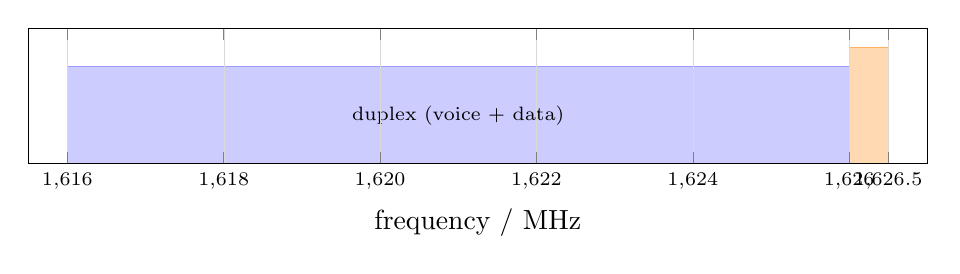
\begin{tikzpicture}
\begin{axis}[
  width=13cm, height=3.3cm,
  xlabel={frequency / MHz},
  ymin=0, ymax=1.4, ytick=\empty,
  xmin=1615.5, xmax=1627,
  xtick={1616, 1618, 1620, 1622, 1624, 1626, 1626.5},
  xticklabel style={font=\scriptsize},
  major grid style={line width=0.1pt,draw=gray!30},
  ymajorgrids=false, xmajorgrids=true,
  axis on top,
]
  % Duplex block
  \addplot[fill=blue!20, draw=blue!40, area legend]
    coordinates {(1616,0)(1616,1)(1626,1)(1626,0)} \closedcycle;
  % Simplex block
  \addplot[fill=orange!30, draw=orange!60, area legend]
    coordinates {(1626,0)(1626,1.2)(1626.5,1.2)(1626.5,0)} \closedcycle;
  \node at (axis cs:1621,0.5) {\scriptsize duplex (voice + data)};
  \node[align=center] at (axis cs:1626.25,1.3) [above] {\tiny simplex};
\end{axis}
\end{tikzpicture}
\end{center}

The centre frequency of channel index $k \in \{0, \ldots, 251\}$ is
\begin{equation}
f_k \;=\; f_{\text{low}} + \left(k + \tfrac{1}{2}\right)\cdot \Delta_{\text{ch}},
\qquad
f_{\text{low}} = \SI{1616}{MHz}, \quad
\Delta_{\text{ch}} = \SI{41.667}{kHz}.
\end{equation}

\subsection{TDMA burst structure and modulation}

Iridium uses time-division multiplex: every \SI{90}{ms} frame is split into
four downlink slots and four uplink slots, plus small guard intervals. Each
slot carries one \emph{burst}: a coherent block of modulated samples of
duration \SI{8.28}{ms} (short burst) up to \SI{20.32}{ms} (long burst).

The modulation is \textbf{differential quaternary phase-shift keying
(DQPSK)} at $R_s = \SI{25}{ksymbols/s}$. Each symbol carries 2 bits;
information is encoded in the \emph{phase difference} between consecutive
symbols, not the absolute phase. The four possible phase differences are
$\{0^\circ, +90^\circ, +180^\circ, -90^\circ\}$, and the sampling
constellation is illustrated below:

\begin{center}
\begin{tikzpicture}[scale=1.4]
  \draw[->] (-1.4,0)--(1.4,0) node[right,font=\scriptsize] {I};
  \draw[->] (0,-1.4)--(0,1.4) node[above,font=\scriptsize] {Q};
  \draw[dashed, gray] (0,0) circle (1);
  % Four symbols
  \fill[blue!70!black] ({cos(45)},  {sin(45)})  circle (0.06)
       node[above right,font=\scriptsize] {\texttt{00}};
  \fill[blue!70!black] ({cos(135)}, {sin(135)}) circle (0.06)
       node[above left,font=\scriptsize] {\texttt{10}};
  \fill[blue!70!black] ({cos(225)}, {sin(225)}) circle (0.06)
       node[below left,font=\scriptsize] {\texttt{11}};
  \fill[blue!70!black] ({cos(315)}, {sin(315)}) circle (0.06)
       node[below right,font=\scriptsize] {\texttt{01}};
\end{tikzpicture}
\captionof{figure}{QPSK constellation used by Iridium (Gray-coded).
Symbols land on $\{\pm 45^\circ, \pm 135^\circ\}$; \emph{differential}
encoding means the mapping shown is applied to the difference between
consecutive symbols, so a static carrier phase offset doesn't matter.}
\end{center}

\subsection{Burst layout}

Every burst begins with a fixed synchronisation pattern that our decoder
looks for:

\begin{center}
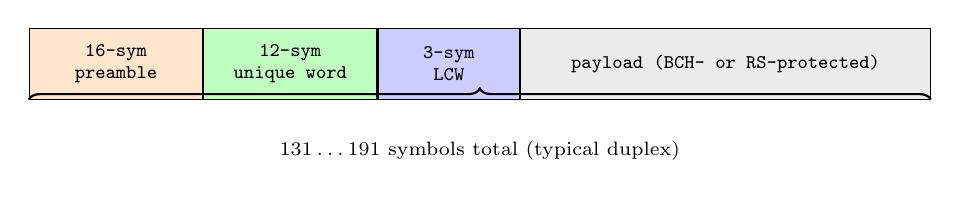
\begin{tikzpicture}[
  seg/.style={draw, minimum height=0.9cm, font=\scriptsize\ttfamily, align=center},
]
  \node[seg, minimum width=2.2cm, fill=orange!20] (preamble)                {16-sym\\preamble};
  \node[seg, minimum width=2.2cm, fill=green!25, right=0 of preamble] (uw)  {12-sym\\unique word};
  \node[seg, minimum width=1.8cm, fill=blue!20,   right=0 of uw] (lcw)      {3-sym\\LCW};
  \node[seg, minimum width=5.2cm, fill=gray!15,   right=0 of lcw] (payload) {payload (BCH- or RS-protected)};

  \draw[decorate, decoration={brace,amplitude=4pt}, thick]
       (preamble.south west) -- (payload.south east)
       node[midway, below=0.4cm, font=\scriptsize]{$131\ldots 191$ symbols total (typical duplex)};
\end{tikzpicture}
\end{center}

The 24-bit \emph{unique word} (UW) after Gray-differential decoding is
\begin{equation}
\text{UW}_{\text{DL}} = \texttt{001100000011000011110011}, \quad
\text{UW}_{\text{UL}} = \texttt{110011000011110011111100}.
\end{equation}
In \emph{symbol} space (before decoding), the same UWs are the fixed
12-symbol patterns
\begin{align}
\text{UW}_{\text{DL}}^\text{sym} &= (0,2,2,2,2,0,0,0,2,0,0,2), \\
\text{UW}_{\text{UL}}^\text{sym} &= (2,2,0,0,0,2,0,0,2,0,2,2).
\end{align}
Both patterns use only symbols $\{0, 2\}$, i.e.\ they are BPSK-symmetric
in the QPSK constellation.

%═══════════════════════════════════════════════════════════════════
\section{Burst Detection (\texttt{FftBurstTagger})}
%═══════════════════════════════════════════════════════════════════

The detector splits the incoming IQ stream into consecutive
$N$-sample FFT frames (typically $N = 2048$ so that each frame covers
$\approx 1$~ms of signal at $f_s = \SI{2}{MHz}$). For each frame it
computes the magnitude-squared spectrum and looks for bins whose energy
significantly exceeds a locally-tracked noise floor.

\subsection{Windowing and FFT}

Frame $m$ is defined as $x_m[n] = x[m N + n]$ for $n = 0, \ldots, N-1$.
Before the DFT it is multiplied by a Blackman window,
\begin{equation}
w[n] \;=\; 0.42 - 0.5\cos\!\left(\frac{2\pi n}{N-1}\right)
         + 0.08\cos\!\left(\frac{4\pi n}{N-1}\right),
\end{equation}
scaled by $1/0.42$ so its DC gain is unity. Windowing reduces spectral
leakage from strong bins into neighbours; Blackman has a stopband
attenuation of $\approx \SI{58}{dB}$.

The frame spectrum is
\begin{equation}
X_m[k] \;=\; \sum_{n=0}^{N-1} x_m[n]\, w[n]\, e^{-j 2\pi k n / N},
\qquad k = 0, \ldots, N-1,
\end{equation}
and its magnitude-squared,
\begin{equation}
P_m[k] \;=\; \bigl|X_m[k]\bigr|^2,
\end{equation}
is the per-bin instantaneous power estimate (unscaled).

\subsection{Adaptive noise floor}

The detector keeps a rolling sum of the last $H = 512$ frame spectra
\emph{that had no active burst}:
\begin{equation}
S[k] \;=\; \sum_{i=1}^{H} P_{m_i}[k], \qquad
\bar{P}[k] \;=\; \frac{S[k]}{H}.
\end{equation}
The relative magnitude of the current frame is then
\begin{equation}
R_m[k] \;=\; \frac{P_m[k]}{S[k]} \;=\; \frac{1}{H}\cdot \frac{P_m[k]}{\bar{P}[k]}.
\end{equation}
A bin is flagged as containing a burst if $R_m[k] > \theta$, where
$\theta$ is derived from the user-set threshold $\gamma$ (in dB) and the
window's equivalent noise bandwidth (ENBW $=1.72$ for Blackman):
\begin{equation}
\theta \;=\; \frac{10^{\gamma / 10}}{H \cdot \mathrm{ENBW}}.
\end{equation}

Because $\bar{P}[k]$ is only updated in frames without active bursts, the
noise-floor estimate does not drift upward during dense passes.

\subsection{Threshold intuition}

For a background of Gaussian noise, $P_m[k]$ is chi-squared distributed
with two degrees of freedom, mean $\bar{P}[k]$. A real Iridium burst
carries $\SI{15}{}\textendash\SI{25}{dB}$ SNR in its centre bin. Setting
$\gamma \in [14, 20]$~dB (default 14) yields a false-alarm rate of a few
per thousand per second while retaining almost all real bursts. This
setting is the \texttt{+/-} key in the plugin.

\begin{center}
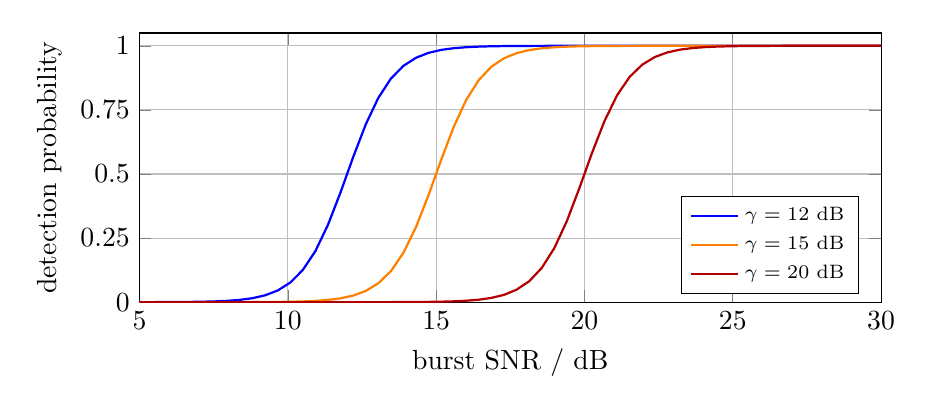
\begin{tikzpicture}
\begin{axis}[
  width=11cm, height=5cm,
  xlabel={burst SNR / dB}, ylabel={detection probability},
  xmin=5, xmax=30, ymin=0, ymax=1.05,
  ytick={0, 0.25, 0.5, 0.75, 1.0},
  grid=both,
  legend pos=south east,
  legend style={font=\scriptsize},
]
  % Q-function approximations for three thresholds
  \addplot[thick, blue,  domain=5:30, samples=60]
    {1 / (1 + exp(-1.3 * (x - 12)))};
  \addlegendentry{$\gamma = 12$~dB}
  \addplot[thick, orange, domain=5:30, samples=60]
    {1 / (1 + exp(-1.3 * (x - 15)))};
  \addlegendentry{$\gamma = 15$~dB}
  \addplot[thick, red!70!black, domain=5:30, samples=60]
    {1 / (1 + exp(-1.3 * (x - 20)))};
  \addlegendentry{$\gamma = 20$~dB}
\end{axis}
\end{tikzpicture}
\captionof{figure}{Illustrative detection probability vs.\ burst SNR for
three threshold settings. Real bursts land at 15\textendash25 dB; a
threshold below the burst SNR catches them, above rejects them.}
\end{center}

\subsection{Burst tracking}

For each bin that is above threshold in the current frame, the detector
either (a) marks an existing burst on that bin as ``still active'' if one
exists, or (b) creates a new burst. A burst is declared ``gone'' if its
centre bin has been below threshold for \texttt{burst\_post\_len} samples
(typically \SI{16}{ms}). Bins within $\pm w/2$ of an active burst are
masked out of the peak search so a single wideband burst produces only
one detection.

\subsection{Output}

For every gone burst the detector emits a tuple
$(t_\text{start}, t_\text{stop}, k_\text{centre}, \text{mag}, \text{noise})$
where $t_\text{start} = m N - \text{burst\_pre\_len}$ is the sample index
$\SI{2}{ms}$ before the first detection frame (so the whole burst,
including preamble, is contained). This is what the downstream stage
consumes.

%═══════════════════════════════════════════════════════════════════
\section{Per-burst Processing (\texttt{BurstDownmix})}
%═══════════════════════════════════════════════════════════════════

Once a burst is extracted, the goal is to (1) shift it to DC, (2) filter
out neighbouring channels, (3) find the burst body and remove the
residual carrier frequency offset (CFO), (4) apply the matched filter,
(5) align the sync-word so demodulation can start at symbol 0.

\subsection{Rough CFO shift}

The detector reports the burst centre bin $k_\text{centre}$; the
corresponding baseband frequency offset is
\begin{equation}
\hat{f}_\text{rough} \;=\; \frac{k_\text{centre} - N/2}{N}\cdot f_s.
\end{equation}
Multiplying the burst by a complex exponential
\begin{equation}
y[n] \;=\; x[n]\, e^{-j 2\pi \hat{f}_\text{rough} n / f_s}
\end{equation}
shifts the burst to \SI{0}{Hz} in baseband.

\subsection{Low-pass filter and decimation}

We design an FIR low-pass with $\pm 20$~kHz passband (i.e.\ half a
burst-width) and \SI{40}{dB} stopband attenuation using the Parks-McClellan
(Remez) algorithm. The Kaiser tap-count estimator sizes the filter to
\begin{equation}
N_\text{taps} \;\approx\; \frac{\alpha - 7.95}{14.36 \cdot \Delta f / f_s} + 1,
\end{equation}
where $\alpha$ is the stopband attenuation in dB and $\Delta f$ the
transition width. For $\alpha = 40$~dB, $\Delta f = \SI{40}{kHz}$,
$f_s = \SI{2}{MHz}$ this gives $N_\text{taps} = 113$.

After filtering, the signal is decimated by
$D = f_s / f_\text{out}$ to the internal working rate
$f_\text{out} = \SI{500}{kHz}$ (giving \texttt{sps}$= 20$ samples per
symbol):
\begin{equation}
z[m] \;=\; (h * y)[m D].
\end{equation}

\subsection{Burst-start detection}

The RRC-filtered burst envelope $|z[m]|^2$ has a distinct rising edge at
the start of the preamble. We smooth it with a narrow low-pass, find the
maximum inside the first \SI{7}{ms}, and take the first index at which
the envelope exceeds $0.28$ times the maximum. A small pre-start guard
(\SI{100}{us}) is subtracted so the RRC transient at the burst edge
doesn't corrupt the CFO estimate.

\subsection{Fine CFO via signal-squared FFT}

Iridium's 16-symbol preamble is BPSK-modulated (all symbols at $s_0 =
-1 - j$ or $s_1 = +1 + j$), so \emph{squaring} the received signal
removes the $\pi$-radian modulation of the preamble and leaves a pure
complex exponential whose frequency is exactly $2\hat{f}_\text{fine}$:
\begin{equation}
u[m] \;=\; z[m]^2 \;\approx\; A\, e^{j 4\pi \hat{f}_\text{fine} m / f_\text{out}} \cdot |s|^2.
\end{equation}
Taking the FFT of $u$ over the preamble+first-UW-symbols window (zero-
padded by a factor of 16 for sub-bin resolution) and finding the peak
bin $k^\star$ gives
\begin{equation}
\hat{f}_\text{fine} \;=\; \frac{k^\star}{2 M}\cdot f_\text{out},
\end{equation}
where $M$ is the padded FFT size. A quadratic peak interpolation refines
$k^\star$ to sub-bin resolution:
\begin{equation}
\Delta k \;=\; \frac{1}{2}\,\frac{\alpha - \gamma}{\alpha - 2\beta + \gamma},
\end{equation}
where $\alpha, \beta, \gamma$ are the magnitudes at bins
$k^\star - 1, k^\star, k^\star + 1$.

\subsection{Root-raised-cosine matched filter}

To maximise SNR at the sampling instants, the receiver applies a
root-raised-cosine (RRC) filter matched to the transmitter's own RRC
pulse-shaper. With roll-off factor $\alpha = 0.4$ and 51 taps at
$f_\text{out} = \SI{500}{kHz}$, the filter's impulse response is
\begin{equation}
h_\text{RRC}(t) = \frac{1}{T_s}\left[
   \frac{\sin\bigl(\pi t (1-\alpha) / T_s\bigr) + 4\alpha (t/T_s)
         \cos\bigl(\pi t (1+\alpha)/T_s\bigr)}
        {\pi t \bigl(1 - (4\alpha t / T_s)^2\bigr) / T_s}
\right],
\end{equation}
sampled at $t = (n - N/2) / f_s$. The taps are normalised to unit DC gain.

\begin{center}
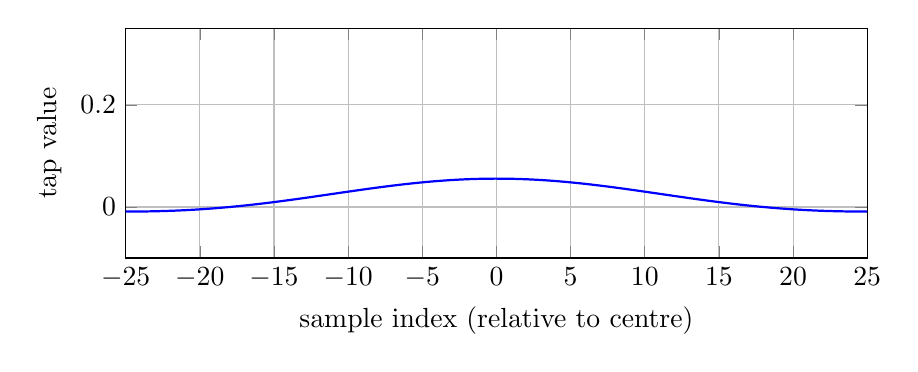
\begin{tikzpicture}
\begin{axis}[
  width=11cm, height=4.5cm,
  xlabel={sample index (relative to centre)}, ylabel={tap value},
  xmin=-25, xmax=25, ymin=-0.1, ymax=0.35,
  grid=both,
]
  \addplot[thick, blue, domain=-25:25, samples=200] {
    (1/20) * (
      sin(deg(3.14159*x/20*(1-0.4))) +
      4*0.4*(x/20)*cos(deg(3.14159*x/20*(1+0.4)))
    )/ ( 3.14159*x/20*(1-(4*0.4*x/20)^2) )
  };
\end{axis}
\end{tikzpicture}
\captionof{figure}{RRC impulse response, $\alpha = 0.4$, sps $= 20$.
Zero-crossings at integer symbol spacings ensure no inter-symbol
interference at the correct sampling instants.}
\end{center}

\subsection{Sync-word alignment}

Even after RRC matched filtering, we still don't know where the burst
starts to sample-level precision. We correlate the received signal with
pre-computed, RRC-shaped versions of both the DL and UL sync-word
templates:
\begin{equation}
c_D[m] \;=\; \sum_{n} z[m+n]\, s_D^\ast[n], \qquad
c_U[m] \;=\; \sum_{n} z[m+n]\, s_U^\ast[n].
\end{equation}
Whichever correlation has the higher peak decides the burst direction
(DL vs UL), and the peak location $m^\star$ tells us where the sync-word
starts. We phase-rotate the burst by $\angle c(m^\star)$ and cut so that
symbol 0 of the aligned frame is the first symbol of the sync-word.

Both correlations are done efficiently by FFT: pre-compute
$\mathcal{F}\{s_D^\ast[-n]\}$ once, then per burst compute
$c_D = \mathcal{F}^{-1}\{\mathcal{F}\{z\} \cdot \mathcal{F}\{s_D^\ast\}\}$.

%═══════════════════════════════════════════════════════════════════
\section{Symbol Demodulation (\texttt{QpskDemod})}
%═══════════════════════════════════════════════════════════════════

\subsection{Symbol-rate decimation}

The aligned burst is at $\texttt{sps} = 20$ samples per symbol. We take
every 20th sample to get one complex value per symbol:
\begin{equation}
r[k] \;=\; z_\text{aligned}[k \cdot \text{sps}].
\end{equation}
This works because RRC pulses have zero-crossings at multiples of the
symbol period so no ISI is introduced.

\subsection{First-order phase-locked loop}

Even after fine CFO correction, small residual phase errors accumulate
across the burst (thermal noise, imperfect fine-CFO estimate). A
first-order QPSK phase-locked loop (PLL) tracks this drift symbol-by-
symbol:
\begin{align}
\hat{r}[k]      &= r[k]\cdot \hat{\varphi}[k]  \\
\hat{s}[k]      &= \text{nearest QPSK symbol of } \hat{r}[k]  \\
e[k]            &= \hat{s}^\ast[k]\cdot \hat{r}[k]  \\
\Delta\phi[k]   &= \alpha \cdot \arg\bigl(e[k] / |e[k]|\bigr)  \\
\hat{\varphi}[k+1] &= e^{-j\Delta\phi[k]}\cdot \hat{\varphi}[k]
\end{align}
The loop constant $\alpha = 1/5$ trades tracking speed vs.\ noise gain.
This is a port of \texttt{gr-burst}'s \texttt{synchronizer\_v4} PLL.

\subsection{QPSK slicer}

The corrected sample $\hat{r}[k]$ is snapped to the nearest quadrant to
produce a hard-decision symbol index $s[k] \in \{0, 1, 2, 3\}$:
\begin{equation}
s[k] \;=\;
\begin{cases}
0 & \text{if } \mathrm{Re}(\hat{r}) \geq 0 \text{ and } \mathrm{Im}(\hat{r}) \geq 0,\\
1 & \text{if } \mathrm{Re}(\hat{r}) < 0   \text{ and } \mathrm{Im}(\hat{r}) \geq 0,\\
2 & \text{if } \mathrm{Re}(\hat{r}) < 0   \text{ and } \mathrm{Im}(\hat{r}) < 0,\\
3 & \text{if } \mathrm{Re}(\hat{r}) \geq 0 \text{ and } \mathrm{Im}(\hat{r}) < 0.
\end{cases}
\end{equation}
The angular offset from the ideal quadrant centre,
$45^\circ - (\text{phase deg}) \bmod 90$, is used to compute
\emph{confidence}: percentage of symbols whose offset $\leq 22^\circ$.
Real Iridium bursts get $50\ldots 70\%$; noise-triggered UW matches get
$25\ldots 40\%$.

\subsection{Unique-word check}

The first 12 symbols of the demodulated sequence should match one of the
two known UW patterns (up to a small number of bit errors from noise).
We use the Hamming distance in \emph{symbol space} with the additional
rule that a symbol difference of $3$ (i.e.\ $270^\circ$) is treated as
$1$ (since $\pm 90^\circ$ errors are indistinguishable):
\begin{equation}
d(\mathbf{s}, \mathrm{UW}) \;=\; \sum_{i=0}^{11}
   \min\bigl(|s_i - \text{UW}_i|,\; 4 - |s_i - \text{UW}_i|\bigr).
\end{equation}
A burst passes the UW check (``A:OK'') if $d \leq 2$ for either the DL or
UL UW.

%═══════════════════════════════════════════════════════════════════
\section{Bit Decoding and Message Parsing}
%═══════════════════════════════════════════════════════════════════

\subsection{Differential Gray decoding}

Because DQPSK encodes information in phase differences, the receiver
computes $b_k = (s_k - s_{k-1}) \bmod 4$ and maps to 2-bit codes via the
Gray table:
\[
\begin{array}{c|c}
b_k & \text{2-bit output}\\ \hline
0 & 00 \\ 1 & 10 \\ 2 & 11 \\ 3 & 01
\end{array}
\]
The output is a bit string of length $2(n-1)$ where $n$ is the number of
demodulated symbols.

\subsection{BCH-protected LCW header}

The 3-symbol \emph{Link Control Word} (LCW) that follows the sync-word
carries the frame type. Iridium protects it with a BCH$(31, 21)$ code
that can correct up to $t = 2$ bit errors. If the received LCW has more
than $t$ errors after Gray-decoding, the frame type is unrecoverable and
the parser emits a \texttt{RAW:} line: unique word recovered but content
unclassifiable.

\subsection{Message classification}

Once the LCW type-code is known, the message is dispatched to a
type-specific parser (IRI, VOC, ISY, IU3, IBC, IME, IRA, \ldots). Each
class has its own field layout, further FEC (Reed-Solomon in some
cases), and interpretation. The vendored \texttt{iridium-toolkit} parser
handles this stage; see the \texttt{plugins/iridium\_decoder/parser/}
directory.

%═══════════════════════════════════════════════════════════════════
\section{End-to-end Block Diagram}
%═══════════════════════════════════════════════════════════════════

\begin{center}
\begin{tikzpicture}[node distance=0.55cm and 0.8cm,
  block/.style={draw, rounded corners, minimum width=3.7cm, minimum height=0.85cm,
                align=center, font=\footnotesize\ttfamily, fill=blue!5},
  stage/.style={draw, dashed, rounded corners=2mm, inner sep=6pt, gray!60},
  lbl/.style={font=\scriptsize\itshape, gray!50!black},
  arrow/.style={-{Latex[length=2mm]}, thick},
]

  \node[block] (fft)      {FFT + Blackman window};
  \node[block, below=of fft]      (mag)  {$|X|^2$ + fftshift};
  \node[block, below=of mag]      (baseline) {baseline moving avg};
  \node[block, below=of baseline] (thr)  {threshold check\\extract peaks};
  \node[block, below=of thr]      (track){track bursts};

  \begin{scope}[on background layer]
    \node[stage, fit=(fft) (mag) (baseline) (thr) (track),
          label={[lbl]above:{FftBurstTagger}}] {};
  \end{scope}

  \node[block, right=1.2cm of fft]        (shift)  {rough shift by $k_c$};
  \node[block, below=of shift]            (lpf)    {LPF + decimate};
  \node[block, below=of lpf]              (start)  {envelope start};
  \node[block, below=of start]            (fine)   {$z^2$ FFT $\to$ fine CFO};
  \node[block, below=of fine]             (rrc)    {RRC matched filter};
  \node[block, below=of rrc]              (sync)   {sync-word FFT-corr};

  \begin{scope}[on background layer]
    \node[stage, fit=(shift) (lpf) (start) (fine) (rrc) (sync),
          label={[lbl]above:{BurstDownmix}}] {};
  \end{scope}

  \node[block, right=1.2cm of shift]      (decsym){decimate to sps};
  \node[block, below=of decsym]           (pll)   {first-order PLL};
  \node[block, below=of pll]              (slice) {QPSK slicer};
  \node[block, below=of slice]            (uw)    {UW check};
  \node[block, below=of uw]               (bits)  {Gray-differential};

  \begin{scope}[on background layer]
    \node[stage, fit=(decsym) (pll) (slice) (uw) (bits),
          label={[lbl]above:{QpskDemod}}] {};
  \end{scope}

  % arrows within each stage
  \draw[arrow] (fft)      -- (mag);
  \draw[arrow] (mag)      -- (baseline);
  \draw[arrow] (baseline) -- (thr);
  \draw[arrow] (thr)      -- (track);
  \draw[arrow] (shift)    -- (lpf);
  \draw[arrow] (lpf)      -- (start);
  \draw[arrow] (start)    -- (fine);
  \draw[arrow] (fine)     -- (rrc);
  \draw[arrow] (rrc)      -- (sync);
  \draw[arrow] (decsym)   -- (pll);
  \draw[arrow] (pll)      -- (slice);
  \draw[arrow] (slice)    -- (uw);
  \draw[arrow] (uw)       -- (bits);

  % stage-to-stage
  \draw[arrow, thick] (track.east) -| ++(0.6, 3) |- (shift.west);
  \draw[arrow, thick] (sync.east)  -| ++(0.6, 3) |- (decsym.west);

  % raw input into tagger
  \node[left=0.3cm of fft, font=\scriptsize] {raw IQ};
  \draw[arrow] ($(fft.west)+(-0.3,0)$) -- (fft.west);

  % output from demod
  \node[right=0.3cm of bits, font=\scriptsize] {bits};
  \draw[arrow] (bits.east) -- ++(0.3,0);

\end{tikzpicture}
\end{center}

%═══════════════════════════════════════════════════════════════════
\section{Performance Considerations}
%═══════════════════════════════════════════════════════════════════

At $f_s = \SI{2}{MHz}$ and $N = 2048$, the tagger runs approximately
\begin{equation}
\frac{f_s}{N} \;\approx\; 977 \text{ FFTs per second}.
\end{equation}
Each FFT costs $O(N \log N) = O(22{,}528)$ operations; per second that is
$\approx 22 \cdot 10^6$ complex multiplies. NumPy's default FFT handles
this in $\approx 100$~ms of CPU per second of data, i.e.\ 10\% of one core.

Per burst, the downmix does one FIR of $\sim 200{,}000 \times 113$ ops
($\SI{22.6}{M}$ ops) plus one FFT of $\sim 4096$ samples for CFO and
another for sync correlation. At a dense-pass rate of $\sim 40$ real
bursts per second, this is $\sim 900 \cdot 10^6$ ops/sec plus $80$
FFT-of-4096 calls. Total CPU usage is 30\textendash 50 \% of a modern
core.

The QPSK PLL and slicer run per symbol (200\textendash 500 symbols per
burst, $\sim 40$ bursts/sec) but each iteration is trivial:
$\sim 10^4$ simple complex operations per second total. In pure Python
these still dominate due to interpreter overhead; with Numba they
become negligible.

Users can toggle the accelerators at runtime:
\begin{itemize}
\item \texttt{n} — Numba JIT for the PLL/slicer loops (off by default;
      on some workloads Numba's per-call dispatch cost outweighs its gain)
\item \texttt{b} — try both bin conventions per burst (2$\times$
      decodes but 2$\times$ downmix cost)
\item \texttt{+}/\texttt{-} — detection threshold up/down by 2~dB
\end{itemize}

The header line in the plugin's message view reports the active backend
combination, e.g.\ \verb|accel: numba* + pyfftw + oaconv|.

%═══════════════════════════════════════════════════════════════════
\section{References}
%═══════════════════════════════════════════════════════════════════

\begin{itemize}
\item \textbf{gr-iridium} — GNU Radio out-of-tree module implementing
      the C++ reference chain (\href{https://github.com/muccc/gr-iridium}{muccc/gr-iridium}).
\item \textbf{iridium-toolkit} — Message parser, extractor scripts, and
      protocol reverse engineering
      (\href{https://github.com/muccc/iridium-toolkit}{muccc/iridium-toolkit}).
\item \textbf{Chaos Communication Congress talks} by Sec \& schneider,
      32C3 (2015) and 33C3 (2016). Reference for the reverse-engineered
      frame formats.
\item \textbf{\emph{Attacks on the Iridium Satellite Network}},
      Groß \& Schafer, WOOT '17.
\item \textbf{\emph{Multirate Signal Processing for Communications
      Systems}}, F.J.\ Harris, 2004 (chs.\ 3, 6, 9 on FIR design and
      polyphase decimation).
\item \textbf{SDRTerm plugin README} —
      \texttt{plugins/iridium\_decoder/README.md} for operational
      details, key bindings, and CLI usage of the plugin.
\end{itemize}

\end{document}
